\section{Caroline - Tech papers}
\subsection{cSculpt: A System for Collaborative Sculpting}
\frame
{
  \frametitle{cSculpt: A System for Collaborative Sculpting}
cSculpt: A System for Collaborative Sculpting \cite{Calabrese:2016}

\begin{figure}
\centering
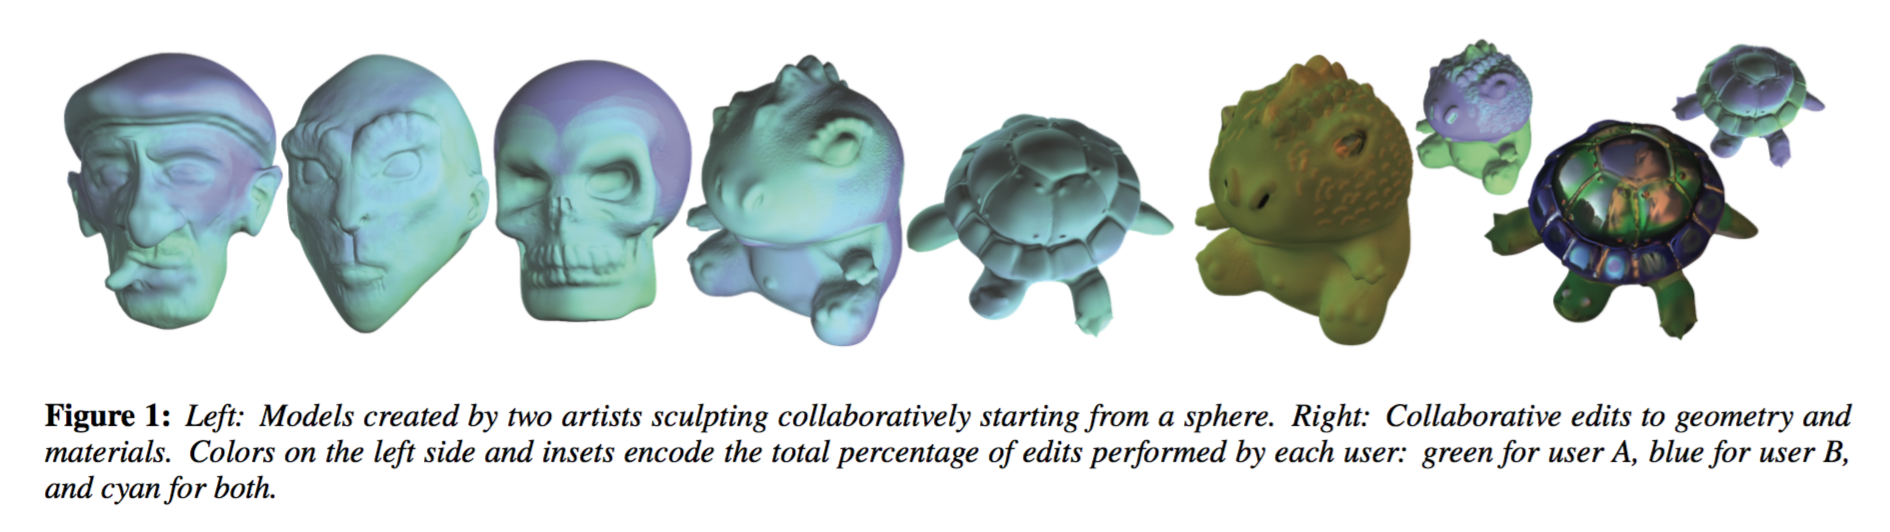
\includegraphics[width=0.9\textwidth]{img/csculpt/summ2.png}
\end{figure}
\centering
\url{https://www.youtube.com/watch?v=H--1zSkarhk}
}
\frame
{
	\frametitle{cSculpt: A System for Collaborative Sculpting}
	\begin{itemize}[<+->]
		\item Context: Unstructured concurrent edit on the same mesh (coarse/fine modifications)
		
		\item Challenge: Multiscale representation $\rightarrow$ edits applied at different spatial frequencies
		
		\item Result: less conflict  == smoother collaboration
		\item Limitation: connectivity updates, scale invariance
	\end{itemize}
}
\frame
{
	\frametitle{cSculpt: A System for Collaborative Sculpting}
	Per-vertex combination for merging multiscale edits
	\begin{figure}
		\centering
		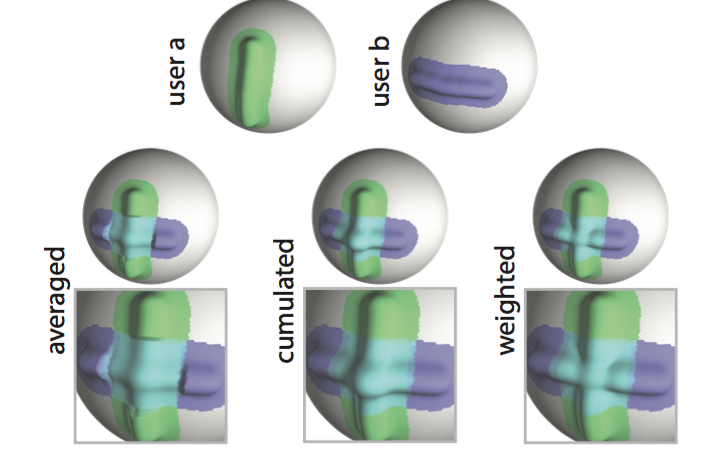
\includegraphics[width=0.3\textwidth]{img/csculpt/combi.png}
		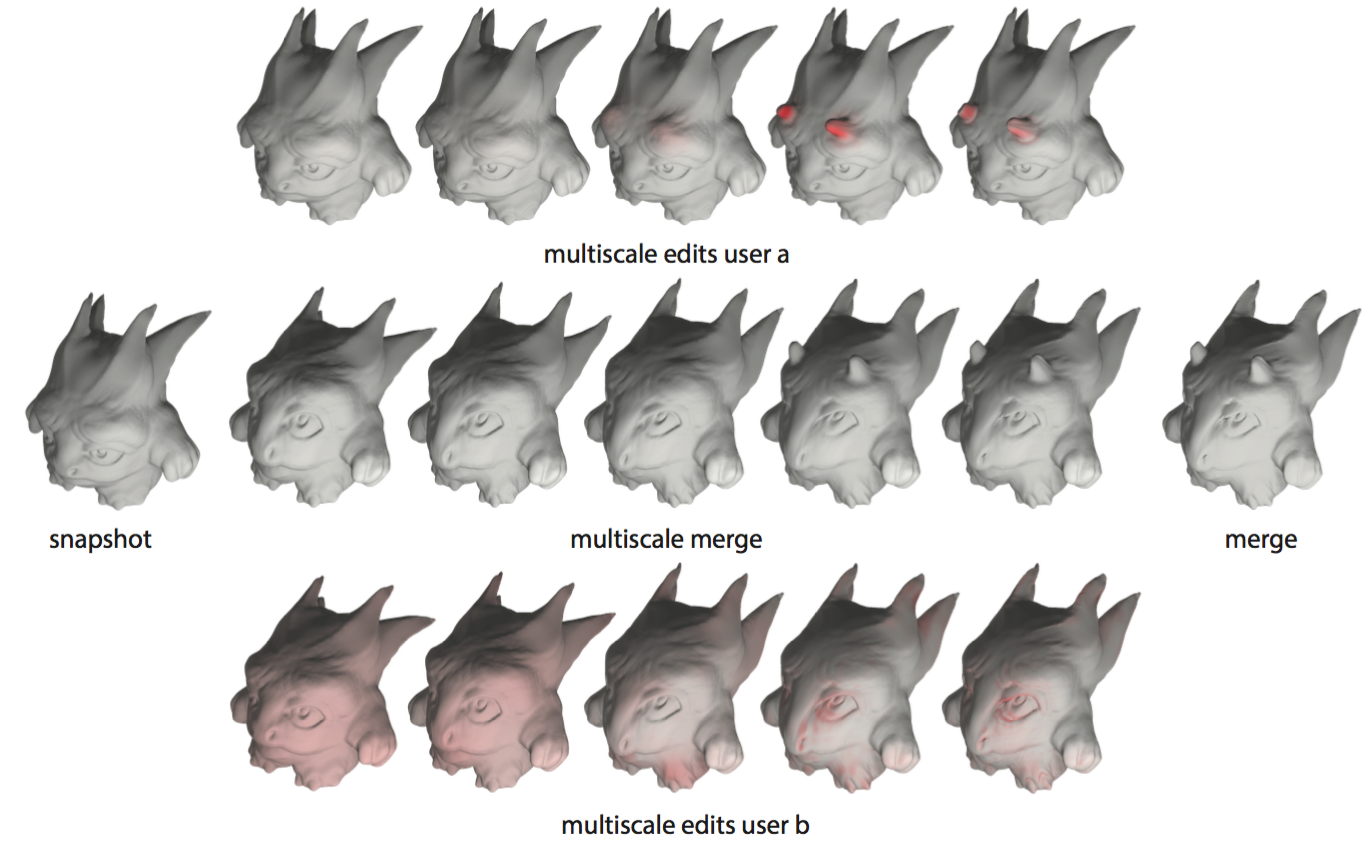
\includegraphics[width=0.6\textwidth]{img/csculpt/merge.png}
	\end{figure}
}


\subsection{Procedural Voronoi Foams for Additive Manufacturing}
\frame
{
	\frametitle{Procedural Voronoi Foams for Additive Manufacturing}
	
	Procedural Voronoi Foams for Additive Manufacturing \cite{Martinez:2016}
	
	\begin{itemize}[<+->]
		\item Context\\
		
		\begin{itemize}
			\item Aperiodic microstructures inspired by Voronoi open-cell foams.
			\item Grade the foam geometry --  and thus its mechanical properties -- within a target object and its surface
		\end{itemize}
		\item Challenges
		\begin{itemize}[<+->]
			\item Fine scale geometry of the strucutres = large scale elastic behavior (global optmization)
			\item Structure's size vs object size = large meshes
			\item Fabricability constraints
		\end{itemize}
		\item Inspiration from procedural noise = infinite contente generated at low cost memory and control statisticlal properties.
	\end{itemize}
	%https://www.youtube.com/watch?v=ENksVUYBrGs
}
\frame
{
	\frametitle{Procedural Voronoi Foams for Additive Manufacturing}
	\begin{itemize}
		\item Contribution
	\begin{itemize}
		\item definition of procedural Voronoi foams that can be evaluated very efficiently, have precisely controlled isotropic elastic behavior, and can be spatially graded to produce gradients of elasticity
		\item methodology to derive an inverse mapping, from a target elasticity to the parameters driving the microstructure generation.
		\item implementation and applications
	\end{itemize}
\end{itemize}
			\begin{figure}
				\centering
				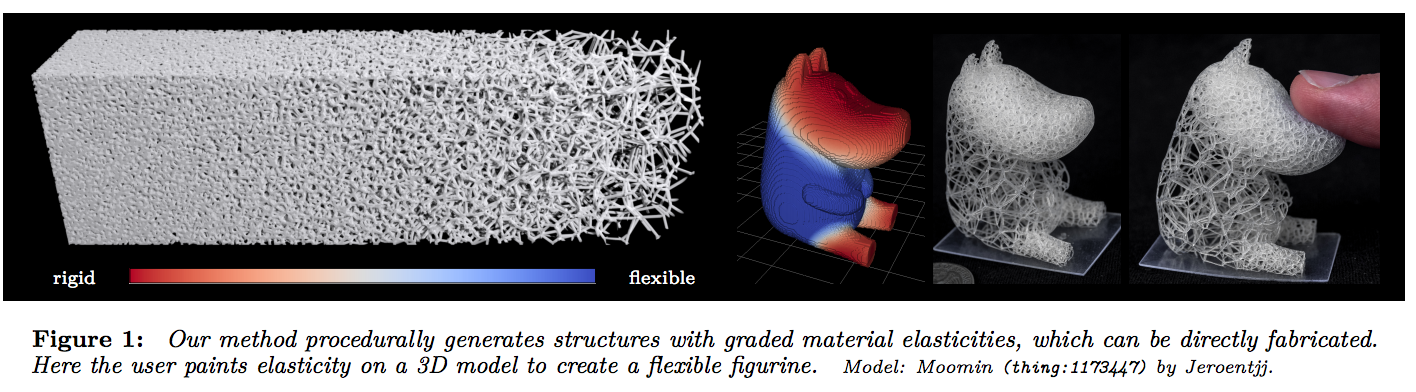
\includegraphics[width=0.9\textwidth]{img/voronoi/headline.png}
			\end{figure}
			\centering
			 \small{\url{https://www.youtube.com/watch?v=ENksVUYBrGs}}
	%https://www.youtube.com/watch?v=ENksVUYBrGs
}

%\frame
%{
%	\frametitle{Procedural Voronoi Foams for Additive Manufacturing}
%Isotropic elastic materials are de- scribed by two parameters: Young’s modulus and Poisson’s ratio. Intuitively the Young’s modulus captures how rigid or soft an object is, while the Poisson’s ratio captures how one dimension stretches with another. In this work we focus on varying the Young’s modulus while preserving the Poisson’s ratio of the base material.
%For spatially varying elasticity we assume the target scalar field is given as input and do not consider its computation.
%	%https://www.youtube.com/watch?v=ENksVUYBrGs
%}

\frame
{
	\frametitle{Procedural Voronoi Foams for Additive Manufacturing}

Procedural voronoi foams generation algorithm, 2 params : 
\begin{itemize}
	\item the density $\rho$ of Voronoi seeds per unit volume (seeds/mm3), 
	\item the radius $\tau$ of the beams along the edges (mm).
\end{itemize}

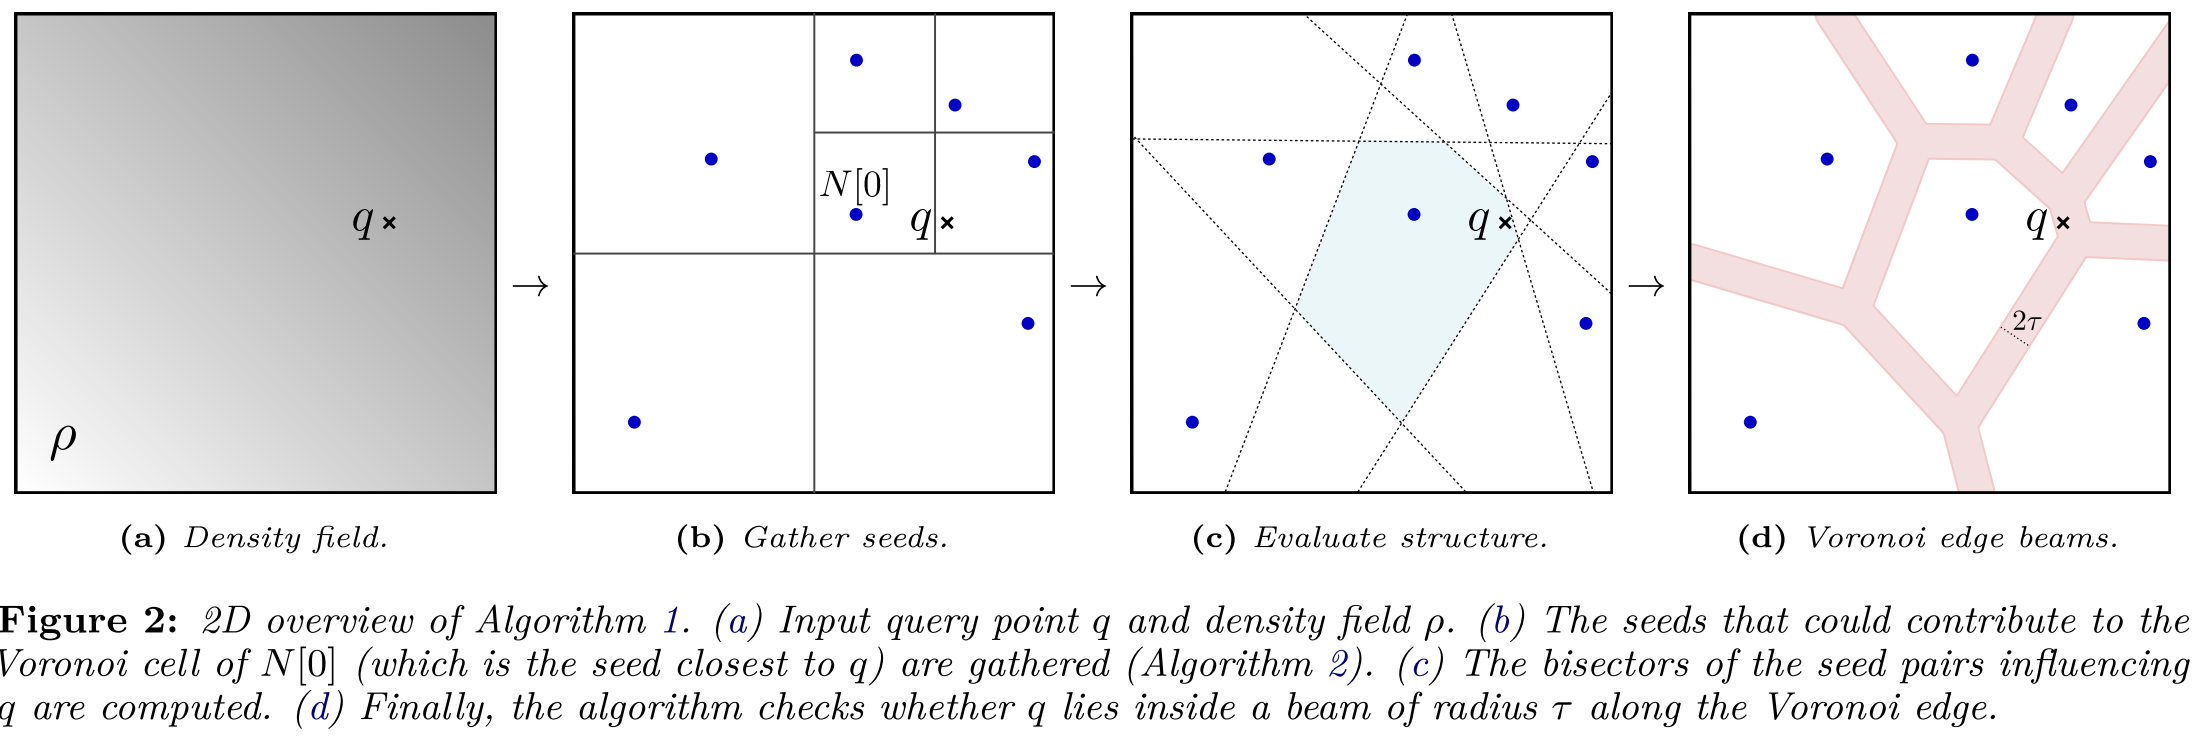
\includegraphics[width=\textwidth]{img/voronoi/algovoronoi.png}

%all grid at least one seed
	%https://www.youtube.com/watch?v=ENksVUYBrGs
}


\subsection{SemanticPaint: Interactive Segmentation and Learning of 3D World}
\frame
{
	\frametitle{SemanticPaint: Interactive Segmentation and Learning of 3D World}
	%https://www.youtube.com/watch?v=z_TcWC7yjj0&feature=youtu.be
	SemanticPaint: Interactive Segmentation and Learning of 3D World \cite{Valentin:2015}
	\begin{figure}
		\centering
		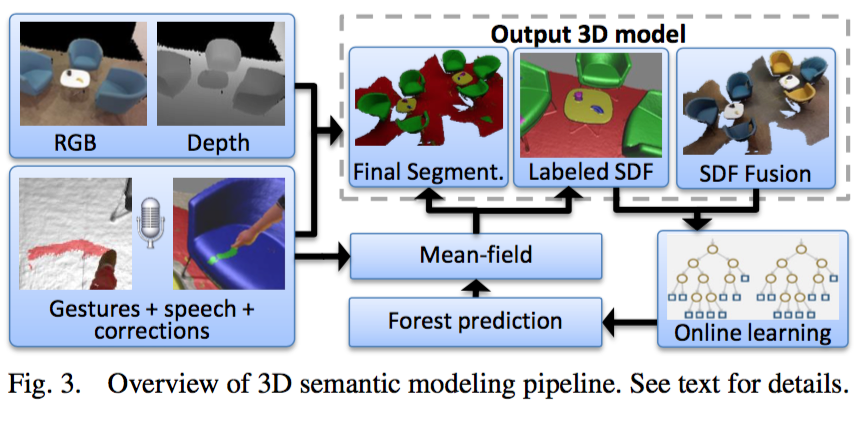
\includegraphics[width=0.9\textwidth]{img/semanticpaint/pipeline.png}
	\end{figure}
	
}
\frame
{
  \frametitle{SemanticPaint: Interactive Segmentation and Learning of 3D World}
%https://www.youtube.com/watch?v=z_TcWC7yjj0&feature=youtu.be

\begin{minipage}[0.2\textheight]{\textwidth}
	\begin{columns}[T]
		\begin{column}{0.5\textwidth}
			
			\begin{itemize}
				\item 3D semantic modeling system
				\item User in the loop $\rightarrow$ online learning
				\item 2 modes: training and test
			\end{itemize}
		\end{column}
		\begin{column}{0.4\textwidth}
			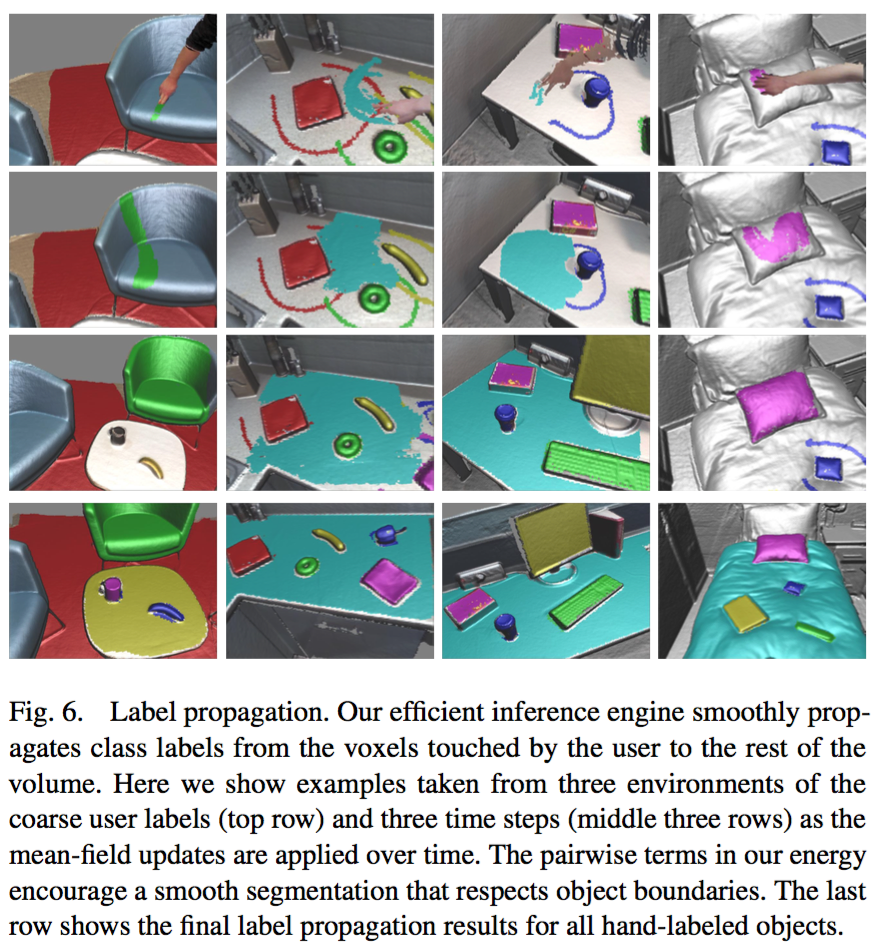
\includegraphics[width=\textwidth]{img/semanticpaint/labelpropagation.png}
		\end{column}
	\end{columns}
\end{minipage}
}

